\documentclass[crop,tikz]{standalone}
\usetikzlibrary{backgrounds}
\colorlet{blue}{cyan}
\tikzset{
  inverted/.style = {
    color=white,
    background rectangle/.style={fill},
    show background rectangle
  }
}

\usepackage{pgfplots}
\tikzset{>=latex}
\usepgfplotslibrary{colormaps}

\begin{document}
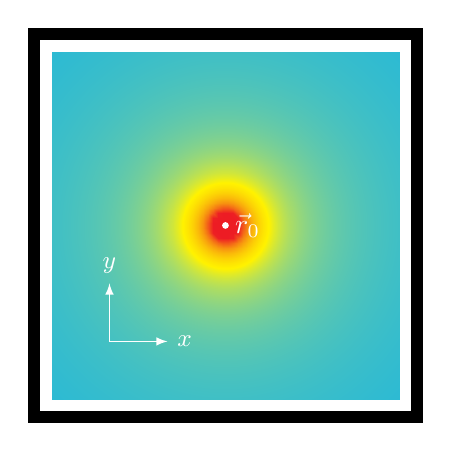
\begin{tikzpicture}[inverted,inverted]
  \begin{axis}[inverted,
    width=6cm,
    height=6cm,
    domain=-3:3,
    shader=interp,
    colormap/hot,
    point meta max=4,
    point meta min=0,
    hide axis,
    zmin=0, zmax=4,
    clip=false,
    declare function = { f(\x,\y) = 1/sqrt(\x^2 + \y^2); },
    view={0}{90},
    ]
    \addplot3[
       restrict z to domain* = 0:4,
       surf,
       samples=70,
    ]{ f(x,y) };
    \addplot3[only marks, mark=*, mark size=1pt] coordinates { (0, 0, 4) } node[right] { $\vec{r}_0$ };
    \coordinate (O) at (axis cs: -2, -2, 0); % origin
    \draw[->, white] (O) -- (axis cs: -1, -2, 0) node[right] { \small $x$ };
    \draw[->, white] (O) -- (axis cs: -2, -1, 0) node[above] { \small $y$ };
  \end{axis}
\end{tikzpicture}
\end{document}
